\section*{Experimental discussion and results}
The neural network used is quite simple so the learning process is not long but the final results can be improved.
To evaluate the quality of a reinforcement learning project, it is not enough to look at the final quality of the model.
It is necessary to evaluate the training time, the response time of the system, and to determine on parameters such as the learning curve if the model can still learn or if it is not the case.

\subsection*{Learning}

It is difficult to visualize neural network learning for reinforcement learning problems.
Especially when using a critical actor.
In fact, if the error on the critic decreases it does not necessarily mean that the actor learns correctly. But it is really the actor who interests us. The error on the actor can be interpreted but it does not allow us to visualize the quality of the policy used by the agent at a given moment t.
To visualize the evolution of an agent in his environment, we must take into account the number of rewards he acquires over time.

\begin{figure}[H]
    \centering
    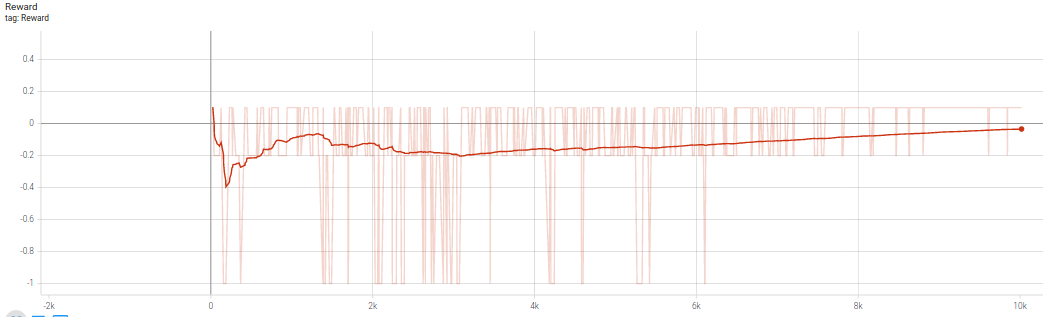
\includegraphics[width=0.5\textwidth]{imgs/reward.png}
    \caption{\label{fig:method} Rewards curve}
\end{figure}

As can be seen on the reward curve the model converges to an acceptable policy after 10K iterations, which is about 5 minutes.
We can consider that the model learned very quickly. 
The environment is quite simple since at first we don't use walls.

\subsection*{Obstacle avoidance}
Our initial goal was to create an agent capable of avoiding all the obstacles he could find.
With the chosen network and the established configuration our agent is able to reach his target avoiding most of the obstacles. 
\begin{figure}[H]
    \centering
    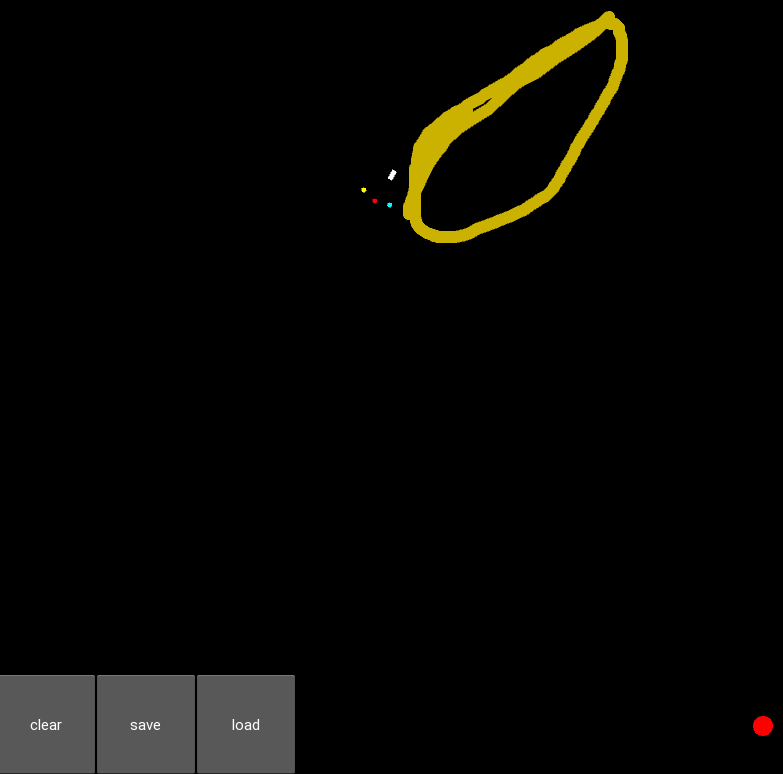
\includegraphics[width=0.1\textwidth]{imgs/obstacle.png}
    \caption{\label{fig:method} Avoiding one Obstacle}
\end{figure}
Even following a path.
\begin{figure}[H]
    \centering
    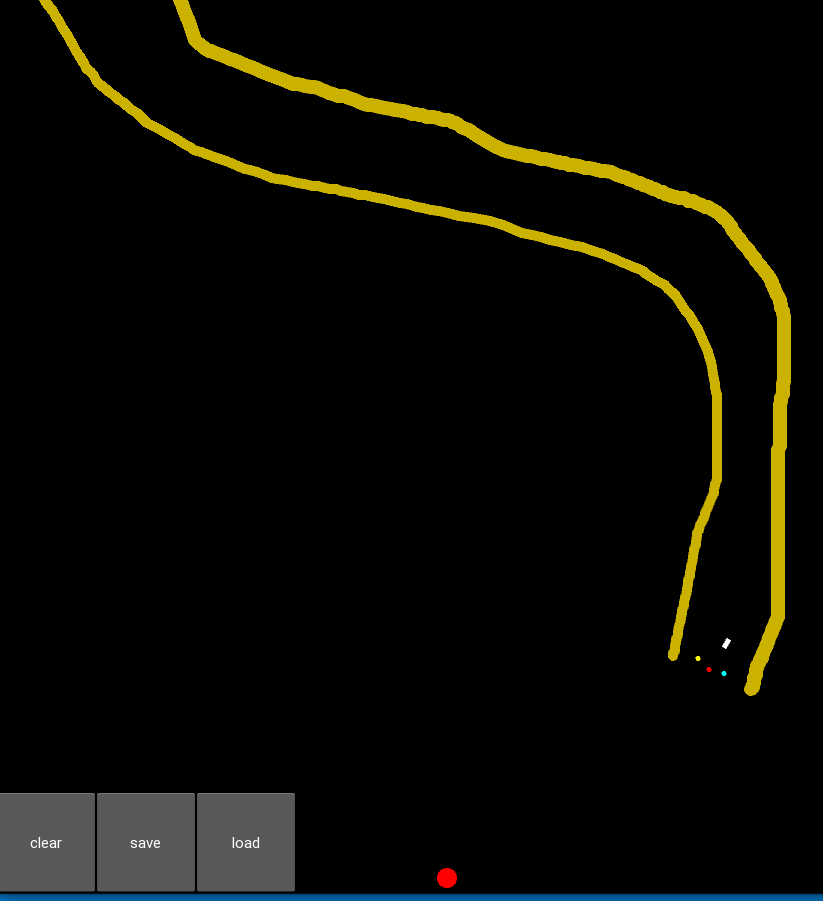
\includegraphics[width=0.1\textwidth]{imgs/path.png}
    \caption{\label{fig:method} Avoiding one Obstacle}
\end{figure}
However in some configurations the robot is sometimes forced to cross the wall to reach the target.
\begin{figure}[H]
    \centering
    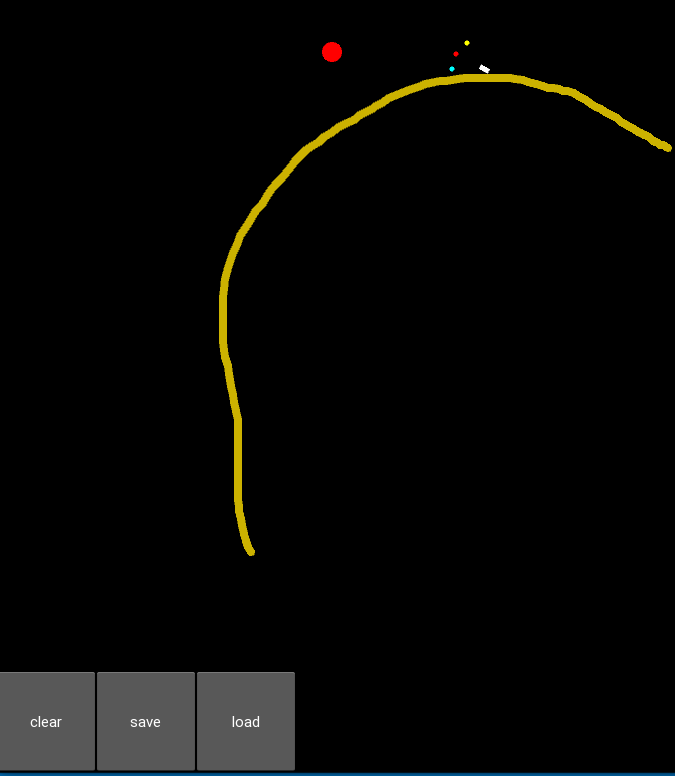
\includegraphics[width=0.1\textwidth]{imgs/U.png}
    \caption{\label{fig:method} The U problem.}
\end{figure}
So if the model presents very good results, it is still perfectible.
To check the results go to : \href{https://github.com/Paul-antoineLeTolguenec/Actor-critic}{Actor-Critic}.

\subsection*{Prospects for improvement}

As the results obtained are the result of a detailed search for the best hyper-parameters of the model (learning rate, gamma, etc.), there are three ways of improving the agent's performance:
\begin{itemize}
    \item \textbf{Building a deeper network}
    One of the possible reasons is that the network that has been built is not sufficient to find the most optimal policy in this Markovian decision process problem.
    One of the solutions is therefore to create a deeper network and thus to add layers of neurons.
    \item \textbf{Add an lstm layer} 
    LSTM \cite{LSTM} are recurrent neural networks. They make it possible to store information in memory. So in case the robot is stuck in a corner, it would be able to know where it comes from. For the moment it only goes with what it sees. Keeping information in memory could probably optimise the robot's performance.
    However, using this type of network leads to problems that can be difficult to solve, such as the vanishing gradient.\cite{vanishing}
    \item \textbf{Implementing another algorithm}
    As we have seen, there are several ways to train a neural network to find the CDM.
    But one of the most optimal methods is the A3C \cite{A3C} algorithm. (asynchronous  advantage  actor-critic)
    This method maximizes the exploration of several agents communicating with each other to find the best policy.
\end{itemize}


\section*{Conclusion}
Our method makes it possible to approximate the CDM and find an acceptable policy. However, the model can still learn. For the moment a more conventional method such as a vector field would work without any doubt.
But the advantage of reinforcement learning methods is that it can be applied to a totally different problem without changing the agent structure and therefore the method.
This is not the case with conventional methods where each problem introduces a new method.

